\documentclass[11pt,a4paper]{article}

% --- Packages ---
\usepackage[utf8]{inputenc}
\usepackage[T1]{fontenc}
\usepackage{lmodern}
\usepackage[margin=1in]{geometry}
\usepackage{graphicx}
\usepackage{xcolor}
\usepackage{hyperref}
\usepackage{booktabs}
\usepackage{tabularx}
\usepackage{amsmath}
\usepackage{fancyhdr}
\usepackage{caption}
\usepackage{subcaption}
\usepackage{tcolorbox}
\usepackage{enumitem}
\usepackage{float}
\usepackage{listings}
\usepackage{microtype}

% --- Graphics Path ---
\graphicspath{{figures/}}

% --- Colors ---
\definecolor{swinburneRed}{RGB}{218, 41, 28}
\definecolor{darkCharcoal}{RGB}{40, 40, 40}
\definecolor{codeBackground}{RGB}{247, 248, 250}
\definecolor{codeBorder}{RGB}{220, 224, 230}
\definecolor{navyBlue}{RGB}{20, 50, 95}
\definecolor{keywordColor}{RGB}{0, 0, 180}
\definecolor{stringColor}{RGB}{163, 21, 21}
\definecolor{commentColor}{RGB}{0, 128, 0}

% --- Hyperref Setup ---
\hypersetup{
    colorlinks=true,
    linkcolor=navyBlue,
    filecolor=navyBlue,      
    urlcolor=swinburneRed,
    citecolor=navyBlue,
    pdftitle={SWE40006 Portfolio Task 1 - Desktop Deployment Using WiX and MSIX},
    pdfauthor={Duc Thanh Le},
    pdfpagemode=FullScreen,
}

% --- Listings Setup ---
\lstset{
    backgroundcolor=\color{codeBackground},
    basicstyle=\ttfamily\footnotesize,
    breaklines=true,
    captionpos=b,
    commentstyle=\color{commentColor},
    keywordstyle=\color{keywordColor}\bfseries,
    stringstyle=\color{stringColor},
    frame=single,
    rulecolor=\color{codeBorder},
    numbers=left,
    numberstyle=\tiny\color{gray},
    numbersep=7pt,
    tabsize=2,
    showstringspaces=false
}

% --- Header and Footer ---
\pagestyle{fancy}
\fancyhf{}
\fancyhead[L]{\small\textcolor{darkCharcoal}{SWE40006 Software Deployment and Evolution}}
\fancyhead[R]{\small\textcolor{darkCharcoal}{Portfolio Task 1: Desktop Deployment}}
\fancyfoot[L]{\small\textcolor{gray}{Duc Thanh Le (Student ID: [Your Student ID])}}
\fancyfoot[R]{\small\thepage}
\renewcommand{\headrulewidth}{0.4pt}
\renewcommand{\footrulewidth}{0.4pt}

% --- Title Block ---
\title{
    \vspace{-1.5cm}
    
\includegraphics[width=0.4\textwidth]{figures/logo.png}\\[1cm]
    \Large \textbf{SWINBURNE UNIVERSITY OF TECHNOLOGY}\\
    \large School of Science, Computing and Engineering Technologies\\[0.5cm]
    \LARGE \textbf{SWE40006 -- Software Deployment and Evolution}\\[0.2cm]
    \huge \textbf{Deployment Portfolio Task 1:}\\
    \LARGE \textbf{Desktop Deployment using Windows Installer XML (WiX) and Modern MSIX Packaging}\\[0.8cm]
}

\author{
    \textbf{Student Name:} Duc Thanh Le \\
    \textbf{Student ID:} 105548505 \\
    \textbf{Lecturer / Assessor:} Tran Minh Hai \\
    \textbf{Repository URL:} \url{https://github.com/[YourUsername]/SWE40006-Portfolio-Task-1}
}

\date{
    \textbf{Due Date:} 28th Sep, 2026 by 11:59 PM \\
    \textbf{Submission Date:} 26th Sep, 2026 \\
    \textbf{Target Level Attempted:} High Distinction (HD -- Tasks 1.1, 1.2, 1.3, 1.4)
}

\begin{document}

\maketitle
\thispagestyle{empty}
\newpage

% --- Table of Contents ---
\tableofcontents
\newpage

% --- Section 1: Declaration & Metadata ---
\section{Task Levels}
Table~\ref{tab:subtasks_overview} summarizes the scope of work executed in this portfolio task.

\begin{table}[H]
\centering
\begin{tabularx}{\textwidth}{l p{4.5cm} c X}
\toprule
\textbf{Sub-Task} & \textbf{Grade Target} & \textbf{Status} & \textbf{Summary of Implemented Work} \\
\midrule
\textbf{Task 1.1} & Pass & Completed & Installed WiX v3.11 toolset and Visual Studio extension; built walkthrough template desktop application; authored \texttt{Product.wxs}; generated and verified MSI installer; packaged into MSIX. \\
\addlinespace
\textbf{Task 1.2} & Credit & Completed & Developed an interactive C\# Windows Forms desktop application (\texttt{demoapp}) featuring dynamic step counting; authored custom WiX deployment script; built standalone MSI and MSIX packages. \\
\addlinespace
\textbf{Task 1.3} & Distinction & Completed & Built a modular Class Library DLL (\texttt{NumberTools.dll}); linked dependency into the UI; updated WiX multi-component installer and MSIX deployment layout. \\
\addlinespace
\textbf{Task 1.4} & High Distinction & Completed & Configured Windows Application Packaging Project (WAP); authored \texttt{Package.appxmanifest}; implemented code signing certificates; documented comprehensive end-to-end Microsoft Store publishing pipeline. \\
\bottomrule
\end{tabularx}
\caption{Declaration and Summary of Sub-Tasks Completed}
\label{tab:subtasks_overview}
\end{table}

\newpage

% --- Section 2: Environment Setup ---
\section{Development and Deployment Environment Setup}
To fulfill the requirements of both legacy Windows Installer (MSI) compilation via WiX and modern application containerization (MSIX), the deployment workstation was configured with the software toolchain documented below.

\begin{itemize}[leftmargin=1.5cm]
    \item \textbf{Integrated Development Environment:} Microsoft Visual Studio 2026 with the .NET Desktop Development workload installed.
    \item \textbf{WiX Toolset Extension:} Visual Studio extension providing WiX project system support, syntax highlighting, and project templates for WiX v3.
    \item \textbf{WiX Toolset v3.11 Build Tools:} Installed via official distribution (\texttt{wix311.exe}).
    \item \textbf{Windows Application SDK / WinUI Packaging Tools:} Utilized in place of deprecated legacy UWP workloads to facilitate Windows Application Packaging (WAP) and generate MSIX application packages instead of APPX.
    \item \textbf{.NET Framework SDK:} Installed .NET Framework 4.7.2 runtime and targeting pack to support compilation of the WinForms client and companion Class Library DLLs.
\end{itemize}

% --- Section 3: Task 1.1 ---
\section{Task 1.1 (Pass): WiX Walkthrough Sample Deployment}

\subsection{Objective and Methodology}
The primary objective of Task 1.1 is to establish a verified baseline for Windows Installer deployments using the declarative Windows Installer XML (WiX) engine. This involves authoring a standard XML deployment definition file (\texttt{Product.wxs}), defining directory tables, features, and components, compiling them into a native \texttt{.msi} package, and exploring modern application packaging using MSIX.

\subsection{Implementation Steps}
\begin{enumerate}[leftmargin=1.2cm]
    \item \textbf{Template Application Creation:} A starter Windows Forms application was created following the unit WiX walkthrough instructions, serving as the sample executable payload (Figure~\ref{fig:t1_sample_app}).
    \item \textbf{WiX Setup Project Authoring:} A WiX Setup Project (\texttt{SetupProject1}) was created within the Visual Studio solution. The XML schema defines:
    \begin{itemize}
        \item \texttt{<Product>}: Defines the product name, unique GUID, version (\texttt{1.0.0.0}), and manufacturer (\texttt{Duc Thanh Le}).
        \item \texttt{<Package>}: Specifies installation scope as \texttt{perMachine} and enables cabinet embedding (\texttt{EmbedCab="yes"}).
        \item \texttt{<Directory>}: Establishes the target filesystem hierarchy under \texttt{ProgramFilesFolder} with an installation folder titled \texttt{DemoAppSoftEval}.
        \item \texttt{<Component>}: Binds the compiled binary to the component GUID and declares the file source macro \texttt{\$(var.demoapp.TargetDir)demoapp.exe}.
    \end{itemize}
    \item \textbf{Compilation and MSI Build:} The WiX toolset compiled the source using \texttt{candle} and linked the database using \texttt{light}, producing the deployment artifact \texttt{SetupProject1.msi} (Figure~\ref{fig:t1_build_success} and Figure~\ref{fig:t1_msi_file}).
    \item \textbf{MSIX Container Packaging:} In modern Windows environments, Win32 apps can be packaged using the Windows Application Packaging Project (WAP). The template application was packaged into an MSIX bundle (Figure~\ref{fig:t1_wap_project}).
    \item \textbf{Installation Verification:} The generated MSIX package was tested via double-click installation, verifying seamless sideloading and registration with the Windows OS shell (Figure~\ref{fig:t1_install_result} and Figure~\ref{fig:t1_msix_created}).
\end{enumerate}

\begin{figure}[H]
    \centering
    \begin{subfigure}[b]{0.48\textwidth}
        \centering
        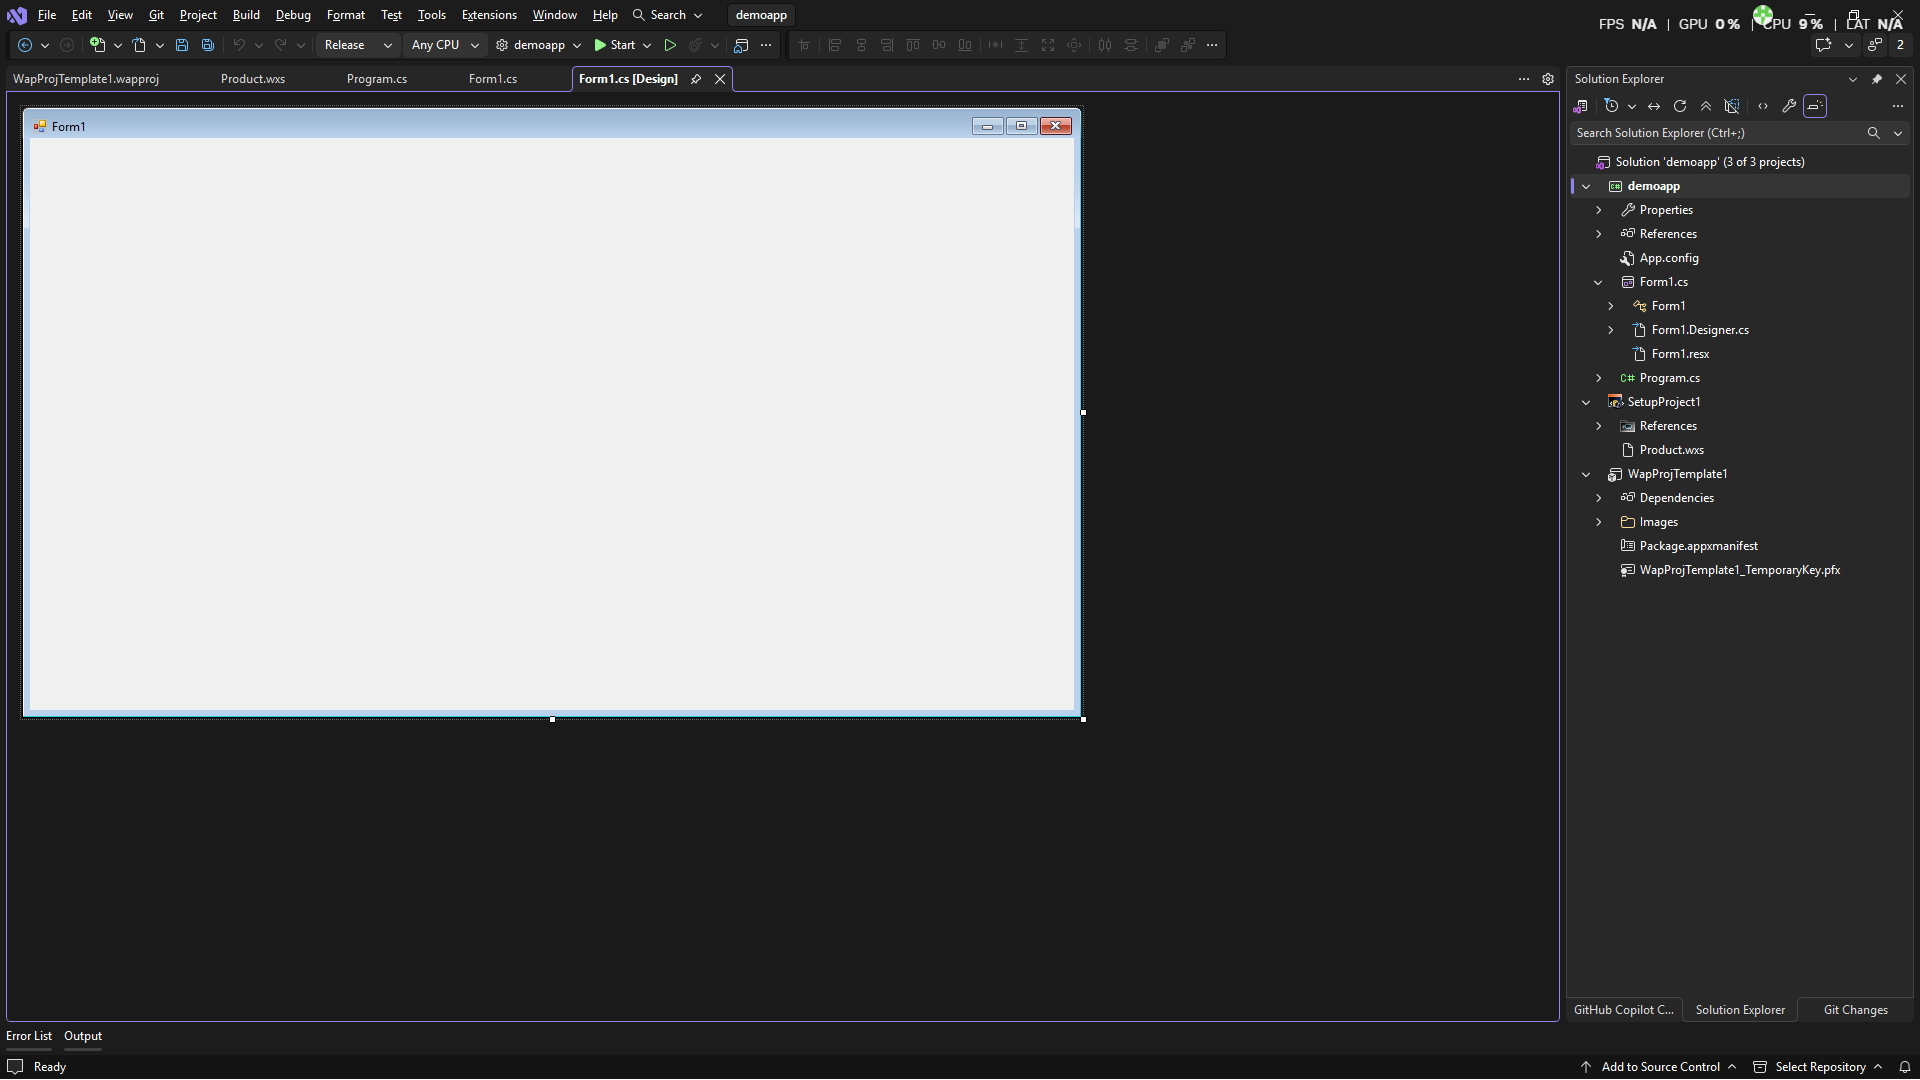
\includegraphics[width=\textwidth]{figures/image4.png}
        \caption{Template Windows Forms desktop application.}
        \label{fig:t1_msi_file}
    \end{subfigure}
    \hfill
    \begin{subfigure}[b]{0.48\textwidth}
        \centering
        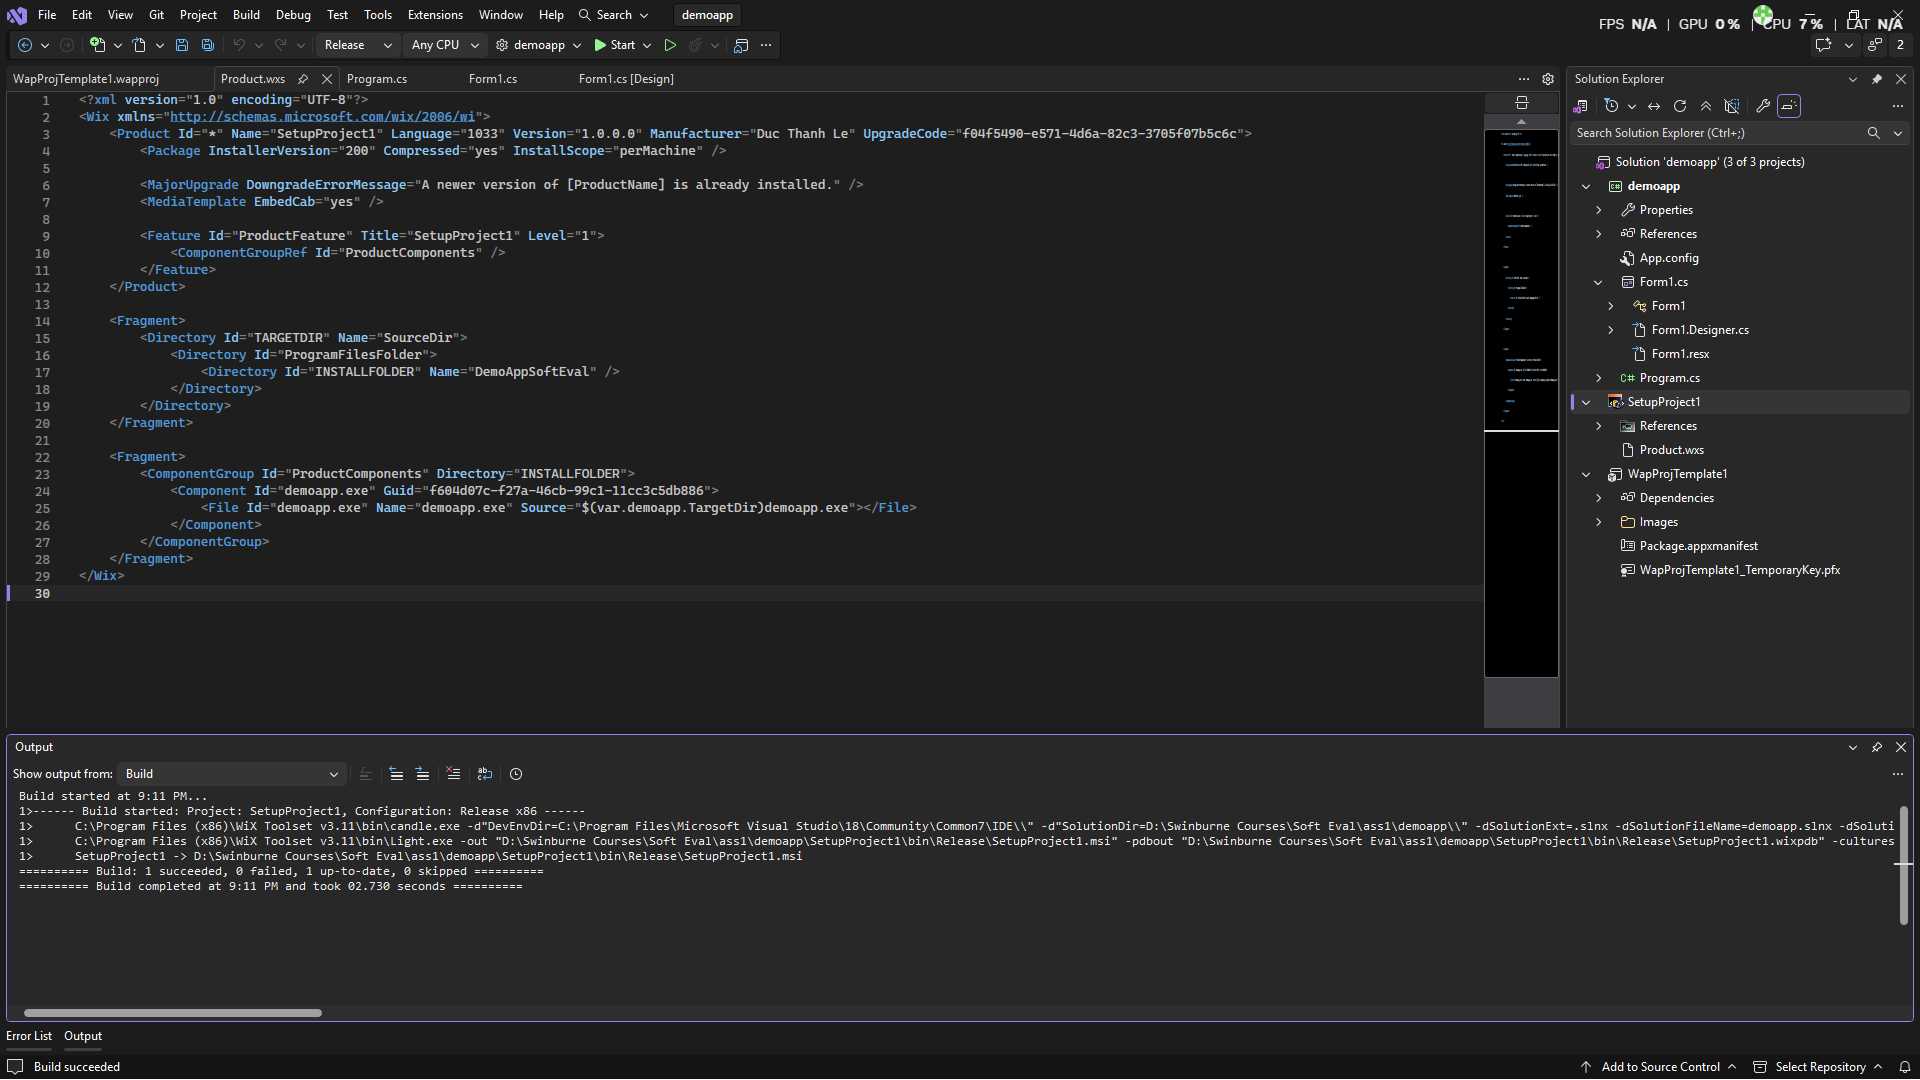
\includegraphics[width=\textwidth]{figures/image5.png}
        \caption{Successful WiX compilation and build output.}
        \label{fig:t1_build_success}
    \end{subfigure}
    \vspace{0.3cm}
    
    \begin{subfigure}[b]{0.48\textwidth}
        \centering
        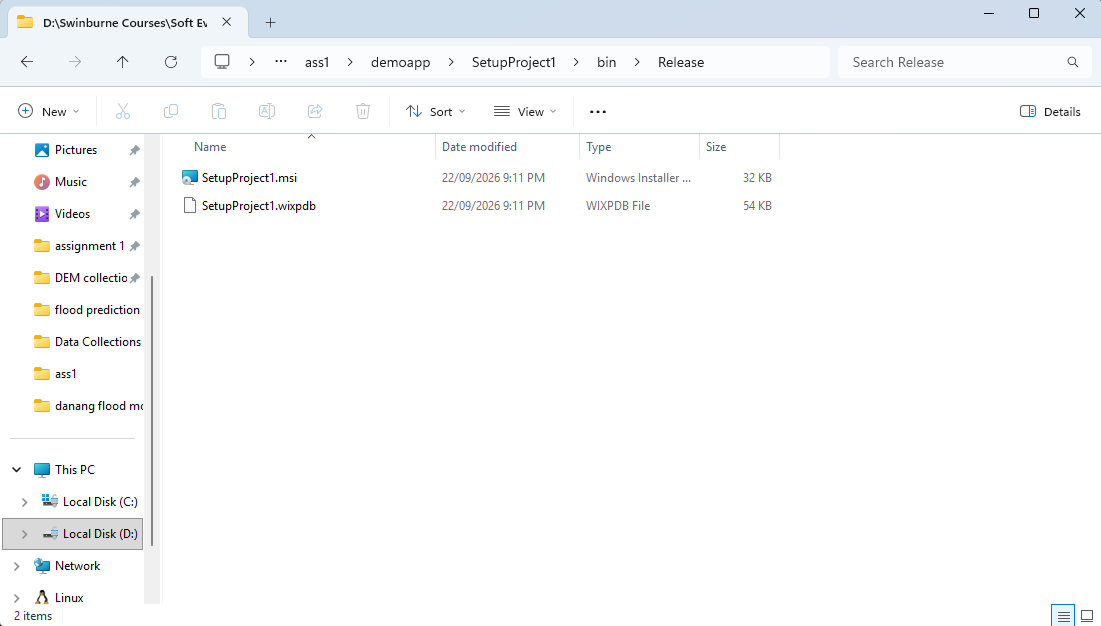
\includegraphics[width=\textwidth]{figures/image6.png}
        \caption{Compiled \texttt{.msi} installer file in Release directory.}
        \label{fig:t1_sample_app}
    \end{subfigure}
    \hfill
    \begin{subfigure}[b]{0.48\textwidth}
        \centering
        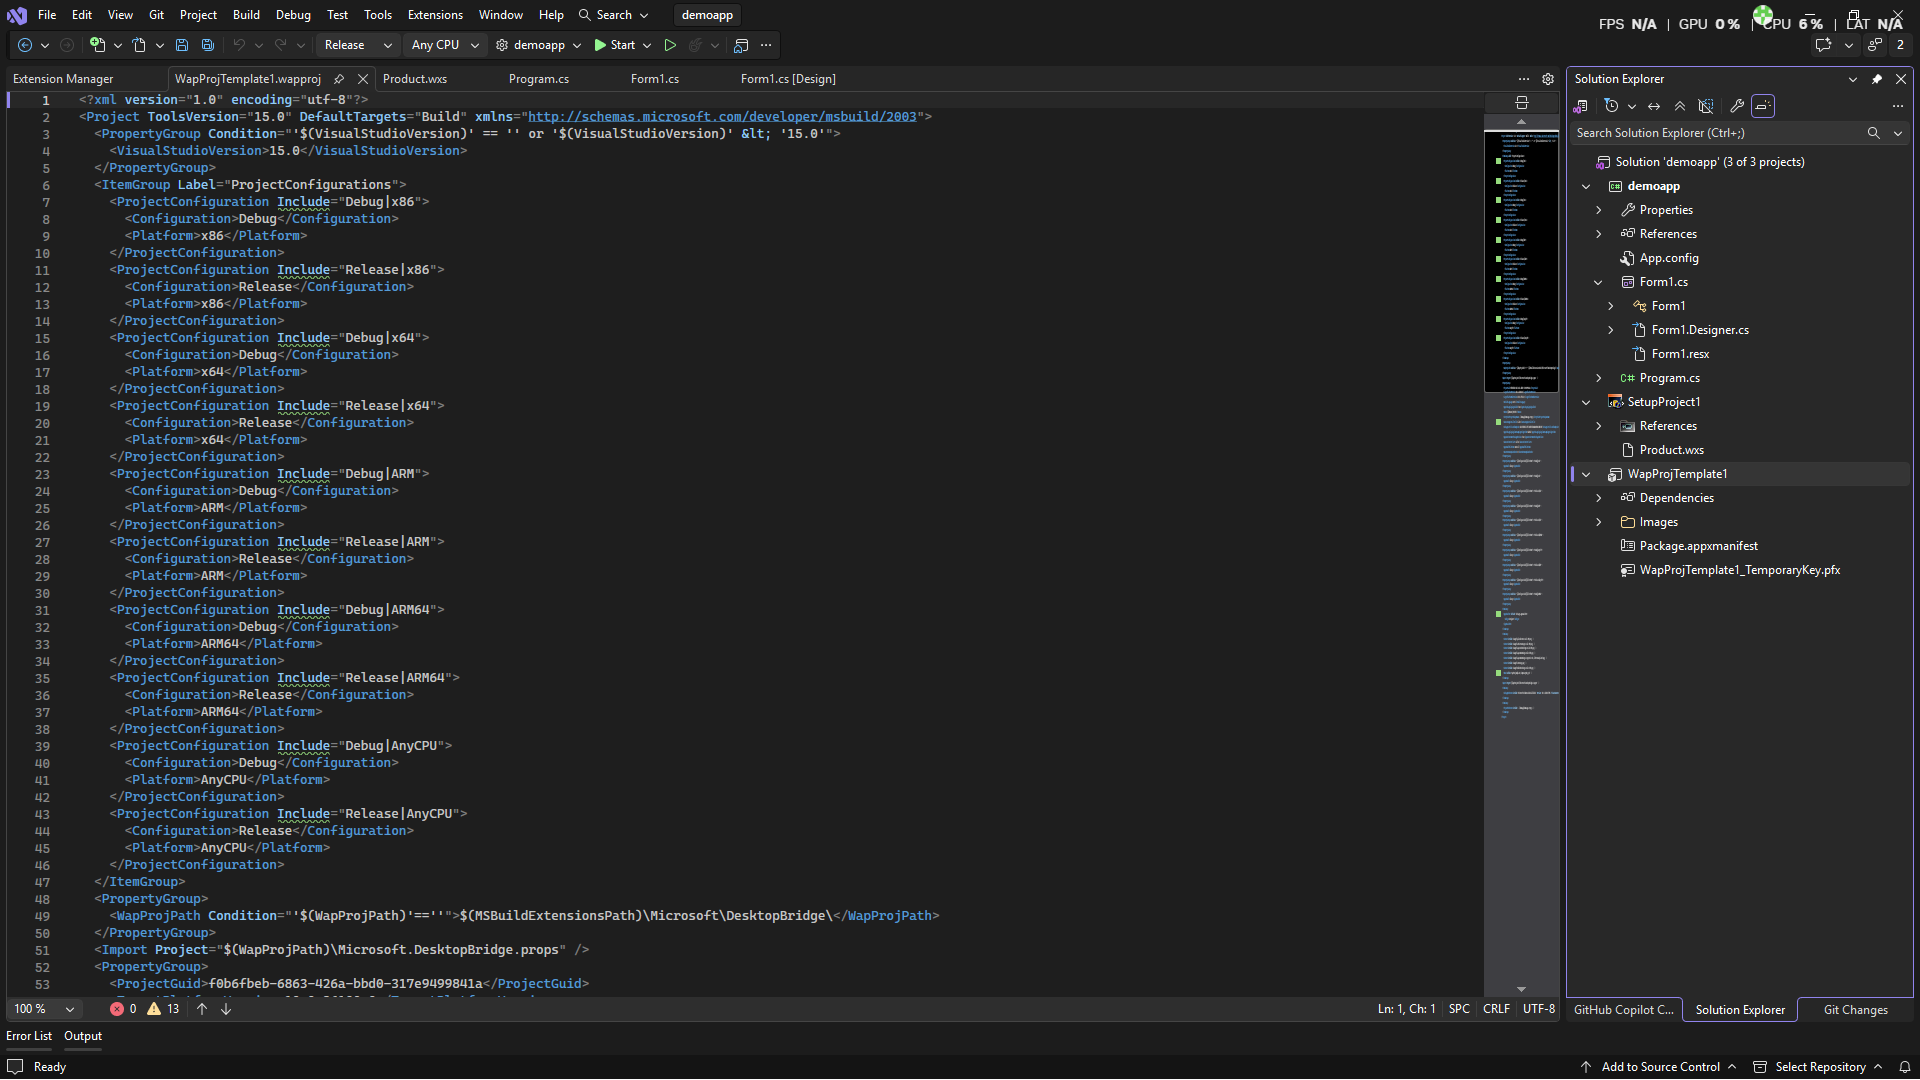
\includegraphics[width=\textwidth]{figures/image8.png}
        \caption{Windows Application Packaging Project (WAP) setup.}
        \label{fig:t1_wap_project}
    \end{subfigure}
    \vspace{0.3cm}
    
    \begin{subfigure}[b]{0.48\textwidth}
        \centering
        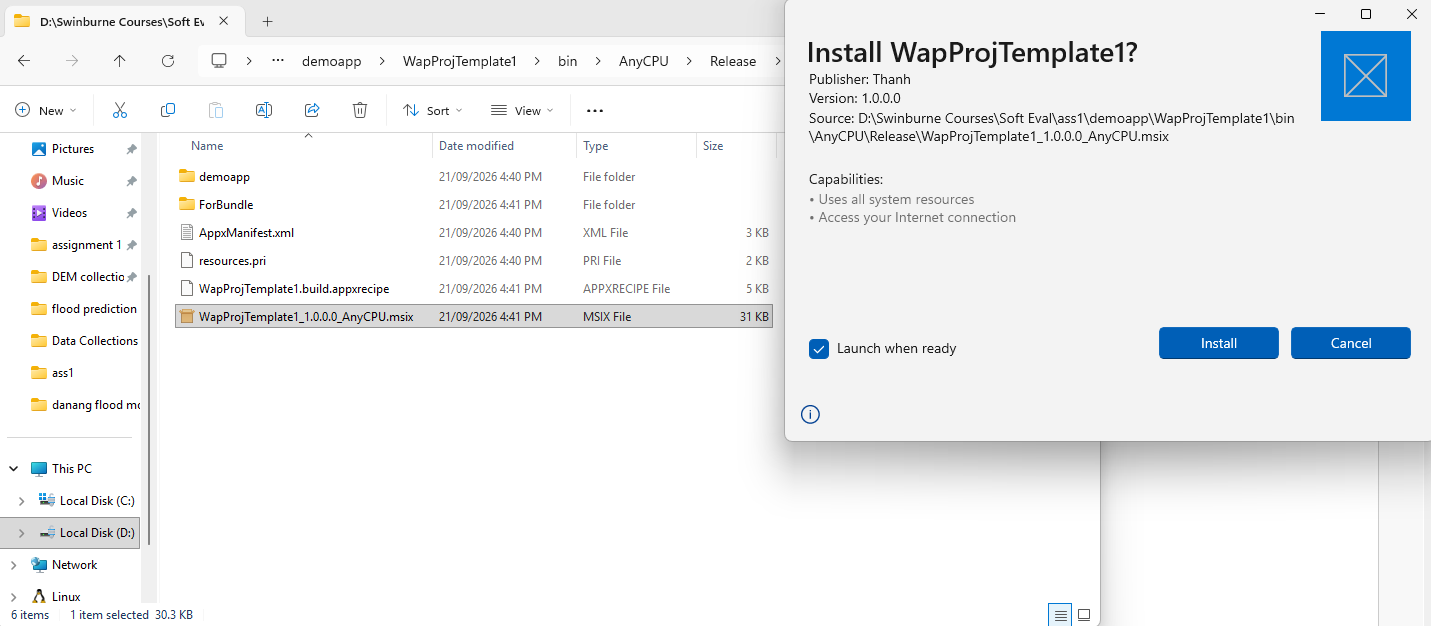
\includegraphics[width=\textwidth]{figures/image9.png}
        \caption{Execution of the completed MSIX installation wizard.}
        \label{fig:t1_install_result}
    \end{subfigure}
    \hfill
    \begin{subfigure}[b]{0.48\textwidth}
        \centering
        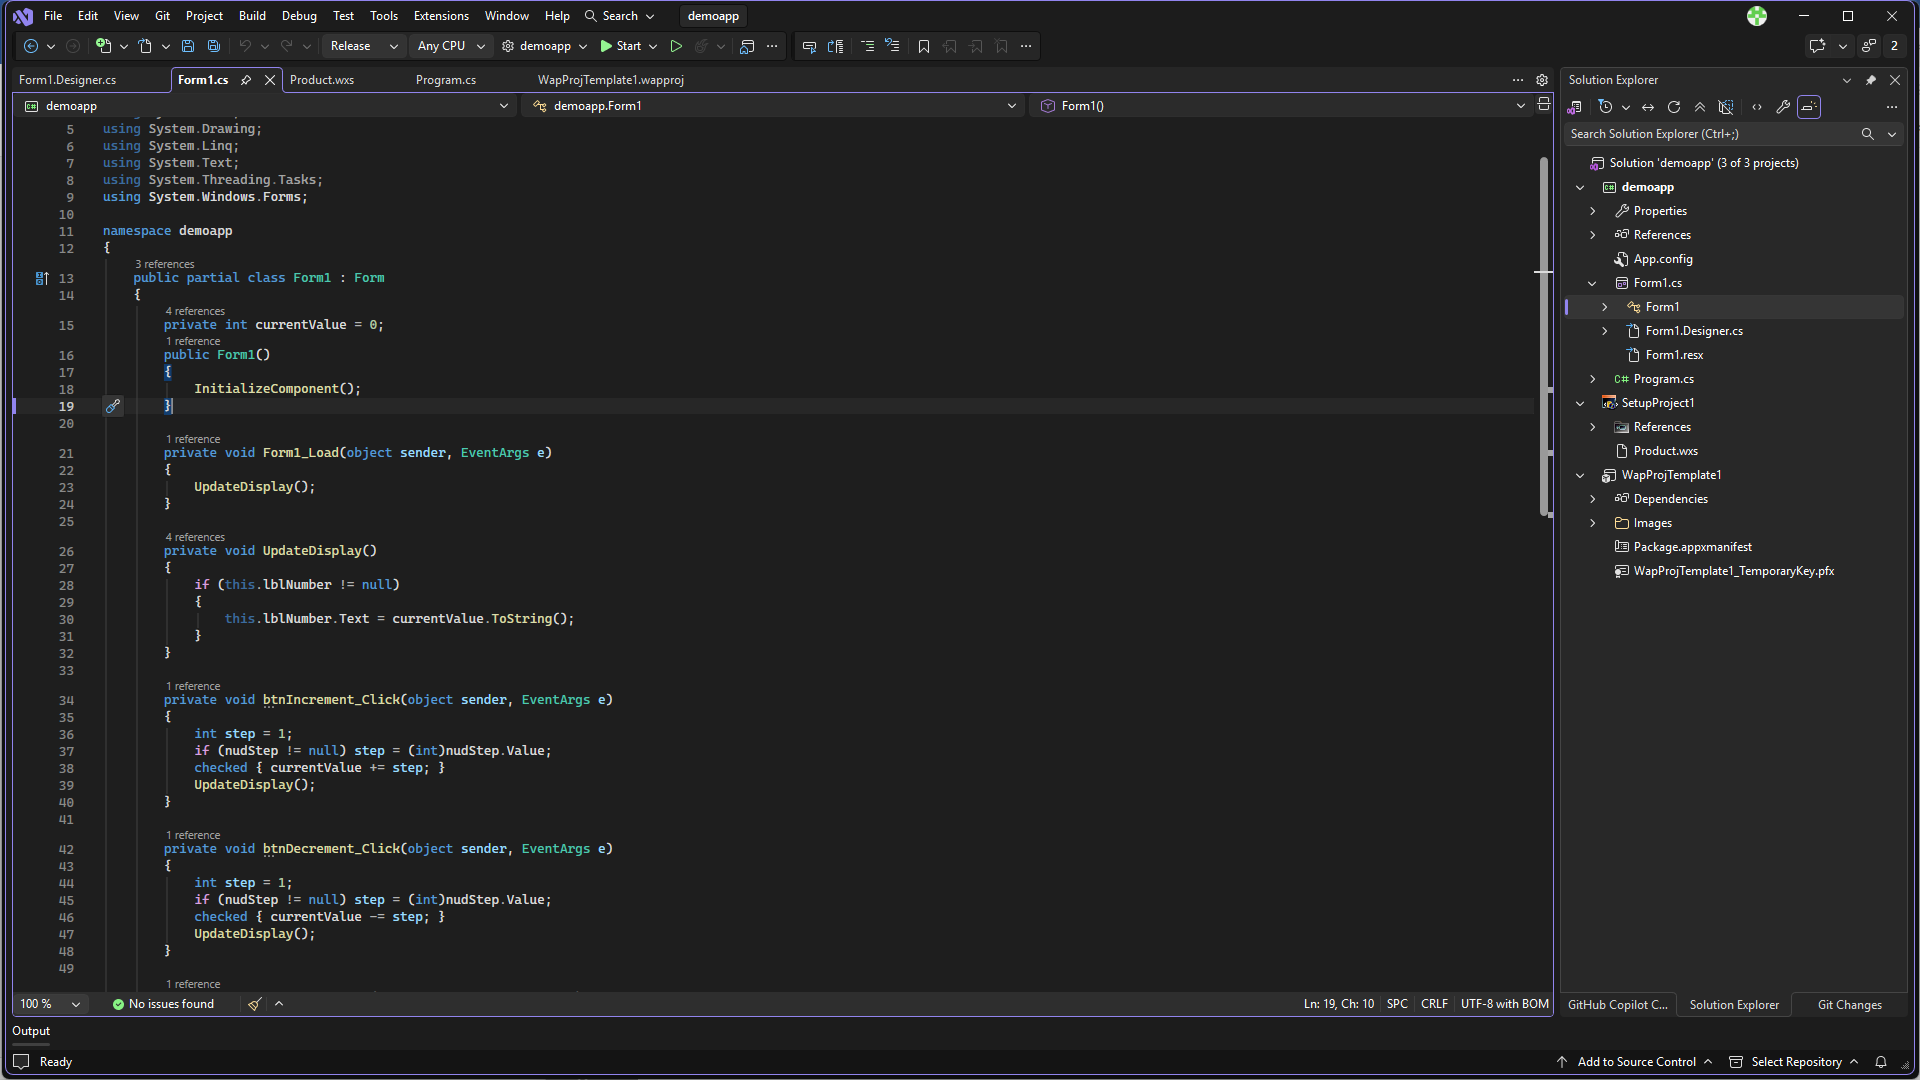
\includegraphics[width=\textwidth]{figures/image10.png}
        \caption{Verified package artifacts ready for deployment.}
        \label{fig:t1_msix_created}
    \end{subfigure}
    \caption{Task 1.1 Deployment Artifacts: WiX MSI and Modern MSIX Verification.}
    \label{fig:task1_evidence}
\end{figure}

\newpage

% --- Section 4: Task 1.2 ---
\section{Task 1.2 (Credit): Custom Desktop Application Deployment}

\subsection{Application Architecture and UI Design}
For Task 1.2, a custom C\# application (\texttt{demoapp}) was created. The application features:
\begin{itemize}[leftmargin=1.5cm]
    \item \textbf{Main Numeric Display (\texttt{lblNumber}):} A central label displaying the current accumulated integer value.
    \item \textbf{Increment/Decrement Controls (\texttt{btnIncrement}, \texttt{btnDecrement}):} Action triggers that modify the accumulator state based on the configured step interval.
    \item \textbf{Customizable Step Selector (\texttt{nudStep}):} A Numeric Up-Down control allowing the end-user to configure custom stepping increments (e.g., $\pm 1, \pm 5, \pm 10$).
    \item \textbf{State Reset Trigger (\texttt{btnReset}):} Instantly restores the internal counter accumulator back to zero.
\end{itemize}

Figure~\ref{fig:t2_codebase} and Figure~\ref{fig:t2_form_design} showcase the codebase structure and design canvas in Visual Studio, while Figure~\ref{fig:t2_app_running} illustrates the running executable.

\begin{figure}[H]
    \centering
    \begin{subfigure}[b]{0.48\textwidth}
        \centering
        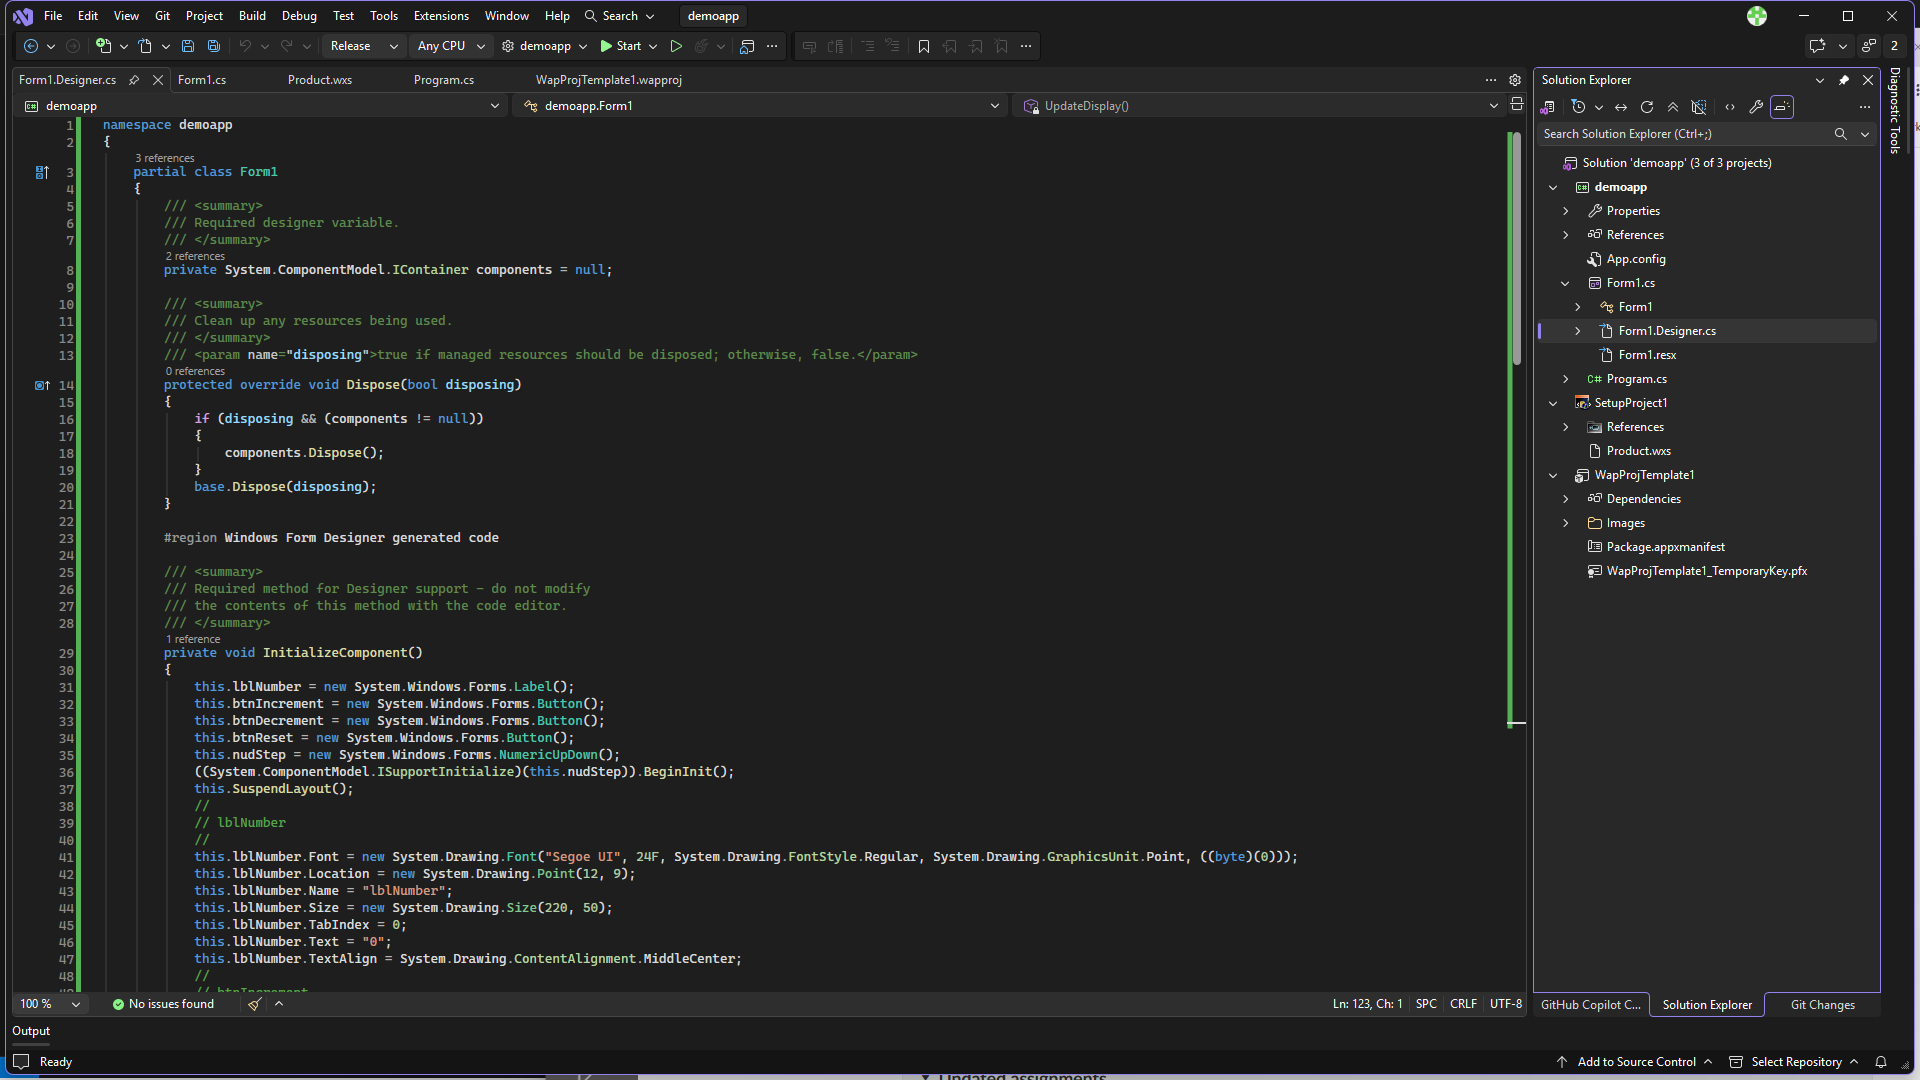
\includegraphics[width=\textwidth]{figures/image11.png}
        \caption{Visual Studio project structure for \texttt{demoapp}.}
        \label{fig:t2_codebase}
    \end{subfigure}
    \hfill
    \begin{subfigure}[b]{0.48\textwidth}
        \centering
        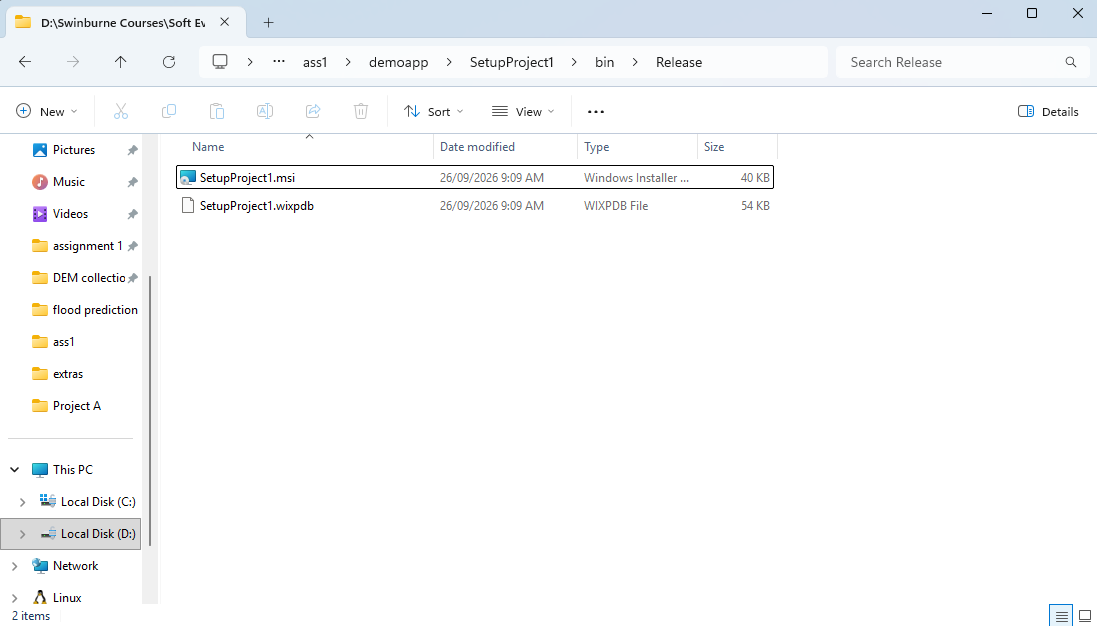
\includegraphics[width=\textwidth]{figures/image12.png}
        \caption{Generated MSI installer (overwrite the blank form application).}
        \label{fig:t2_form_design}
    \end{subfigure}
    \vspace{0.3cm}
    
    \begin{subfigure}[b]{0.48\textwidth}
        \centering
        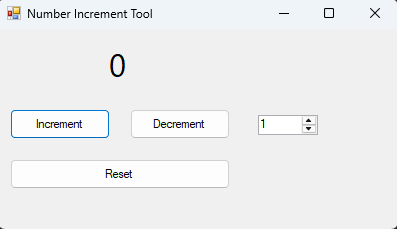
\includegraphics[width=0.75\textwidth]{figures/image13.png}
        \caption{Running custom application featuring step-setting controls.}
        \label{fig:t2_app_running}
    \end{subfigure}
    \hfill
    \begin{subfigure}[b]{0.48\textwidth}
        \centering
        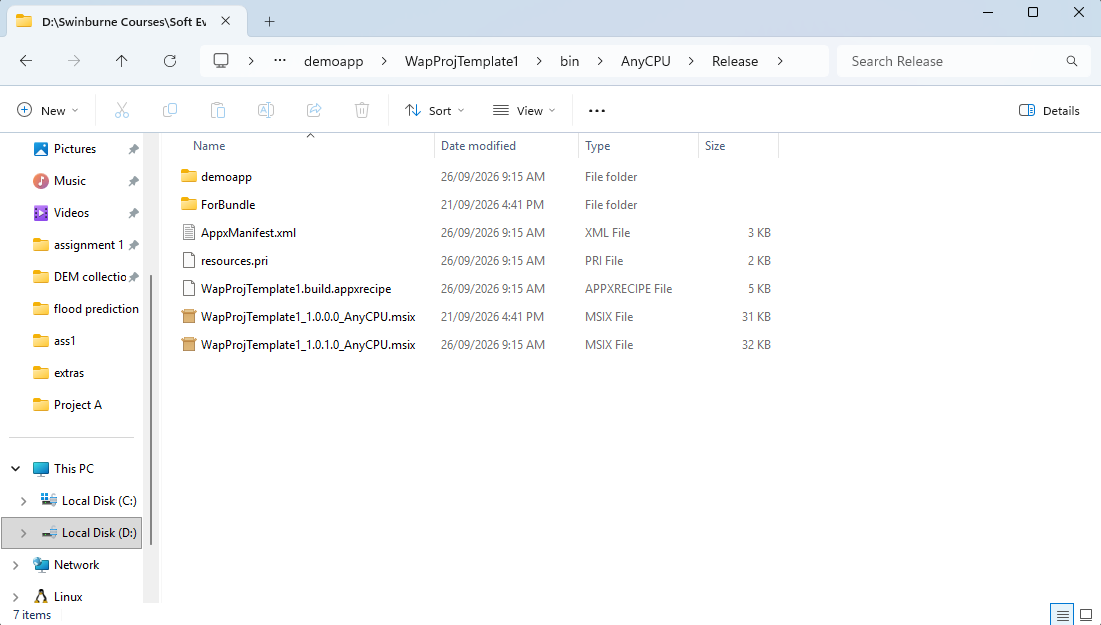
\includegraphics[width=\textwidth]{figures/image15.png}
        \caption{New MSIX file for custom app.}
        \label{fig:t2_msix_pack}
    \end{subfigure}
    \caption{Task 1.2 Custom Application Development and Deployment Artifacts.}
    \label{fig:task2_evidence}
\end{figure}

\subsection{WiX and MSIX Deployment Execution}
The custom executable \texttt{demoapp.exe} was integrated into the WiX setup definition. A clean upgrade code GUID was allocated, and the project reference was linked. Additionally, the Windows Application Packaging Project was updated to bundle \texttt{demoapp.exe}, producing an updated MSIX package.

\newpage

% --- Section 5: Task 1.3 ---
\section{Task 1.3 (Distinction): Custom DLL Implementation and Multi-Dependency Deployment}

\subsection{Implementation of the \texttt{NumberTools} Class Library}
A separate C\# Class Library project named \texttt{NumberTools} was created within the Visual Studio solution. The core logic was encapsulated into the \texttt{NumberCounter} class (Figure~\ref{fig:t3_custom_dll} and Listing~\ref{lst:numbercounter}).

\begin{lstlisting}[language={[Sharp]C}, caption={\texttt{NumberCounter.cs} Class Library Implementation}, label={lst:numbercounter}]
namespace NumberTools
{
    public class NumberCounter
    {
        public int Value { get; private set; }

        public void Increment(int amount)
        {
            checked { Value += amount; }
        }

        public void Decrement(int amount)
        {
            checked { Value -= amount; }
        }

        public void Reset()
        {
            Value = 0;
        }
    }
}
\end{lstlisting}

Compilation of \texttt{NumberTools.csproj} produces the binary artifact \texttt{NumberTools.dll} (Figure~\ref{fig:t3_actual_dll}).

\subsection{Client Integration and Dependency Linking}
The client desktop application (\texttt{demoapp}) was updated to consume the external DLL:
\begin{enumerate}[leftmargin=1.2cm]
    \item An Assembly/Project Reference was added from \texttt{demoapp} to \texttt{NumberTools} (Figure~\ref{fig:t3_ref_project}).
    \item The client namespace imported \texttt{using NumberTools;}.
    \item All state mutations were delegated to an instantiated instance of \texttt{NumberCounter} (Figure~\ref{fig:t3_new_code} and Listing~\ref{lst:form1}).
\end{enumerate}

\begin{figure}[H]
    \centering
    \begin{subfigure}[b]{0.48\textwidth}
        \centering
        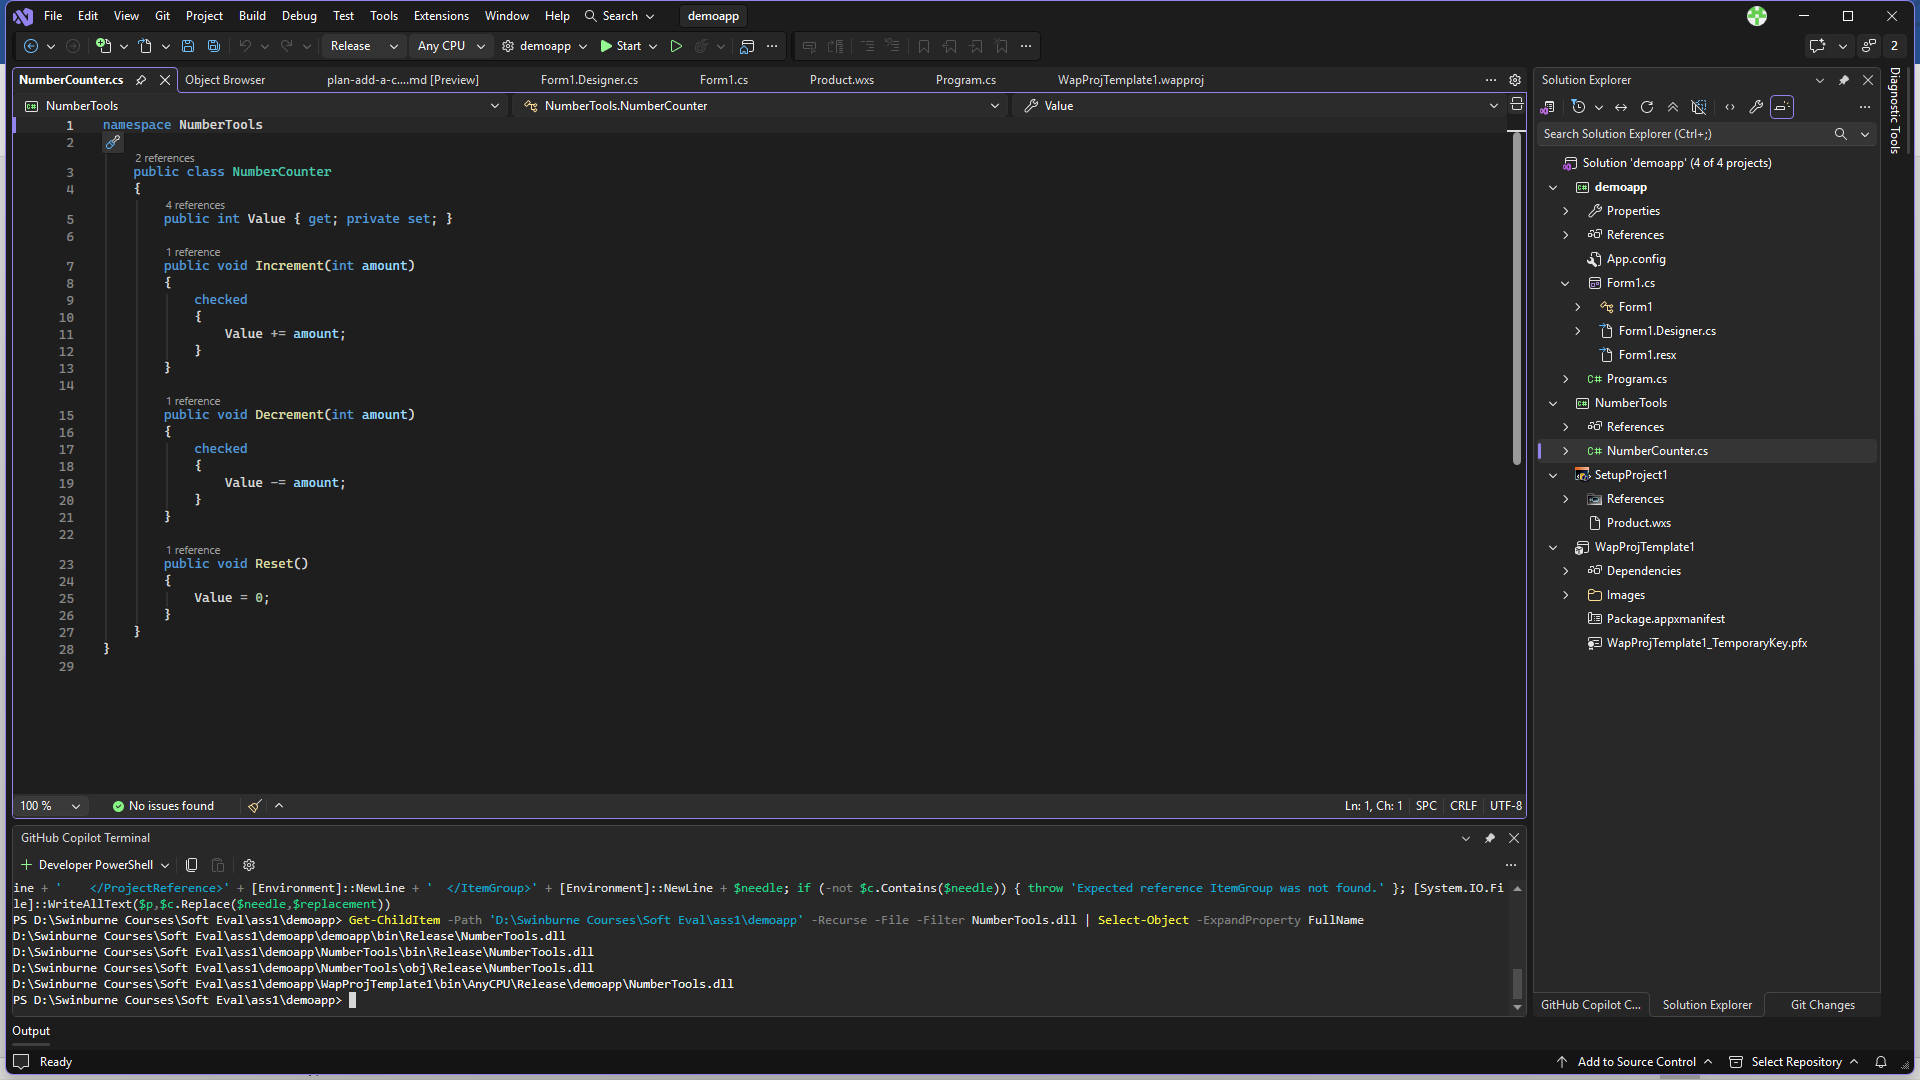
\includegraphics[width=\textwidth]{figures/image16.png}
        \caption{Creation of the \texttt{NumberTools} Class Library project.}
        \label{fig:t3_custom_dll}
    \end{subfigure}
    \hfill
    \begin{subfigure}[b]{0.48\textwidth}
        \centering
        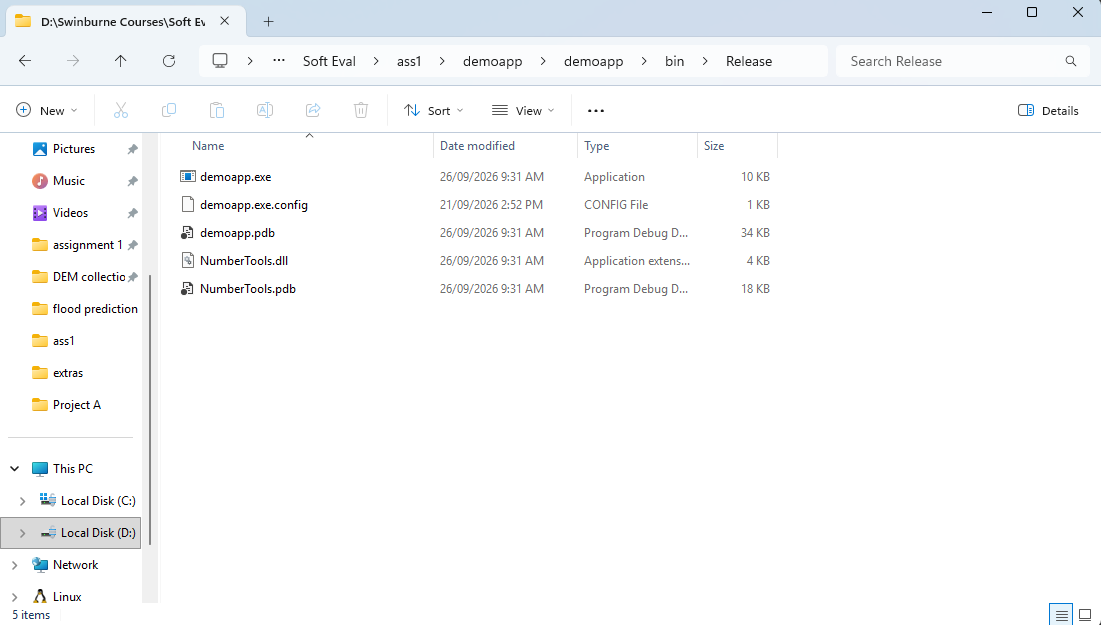
\includegraphics[width=\textwidth]{figures/image17.png}
        \caption{Compiled \texttt{NumberTools.dll} binary artifact in Release folder.}
        \label{fig:t3_actual_dll}
    \end{subfigure}
    \vspace{0.3cm}
    
    \begin{subfigure}[b]{0.48\textwidth}
        \centering
        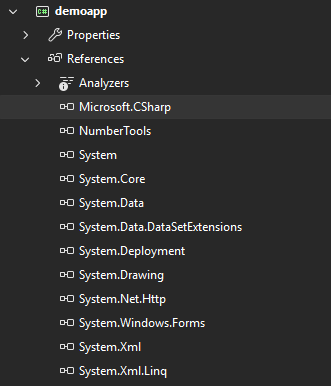
\includegraphics[width=0.65\textwidth]{figures/image18.png}
        \caption{Assembly reference to \texttt{NumberTools.dll} in client app.}
        \label{fig:t3_ref_project}
    \end{subfigure}
    \hfill
    \begin{subfigure}[b]{0.48\textwidth}
        \centering
        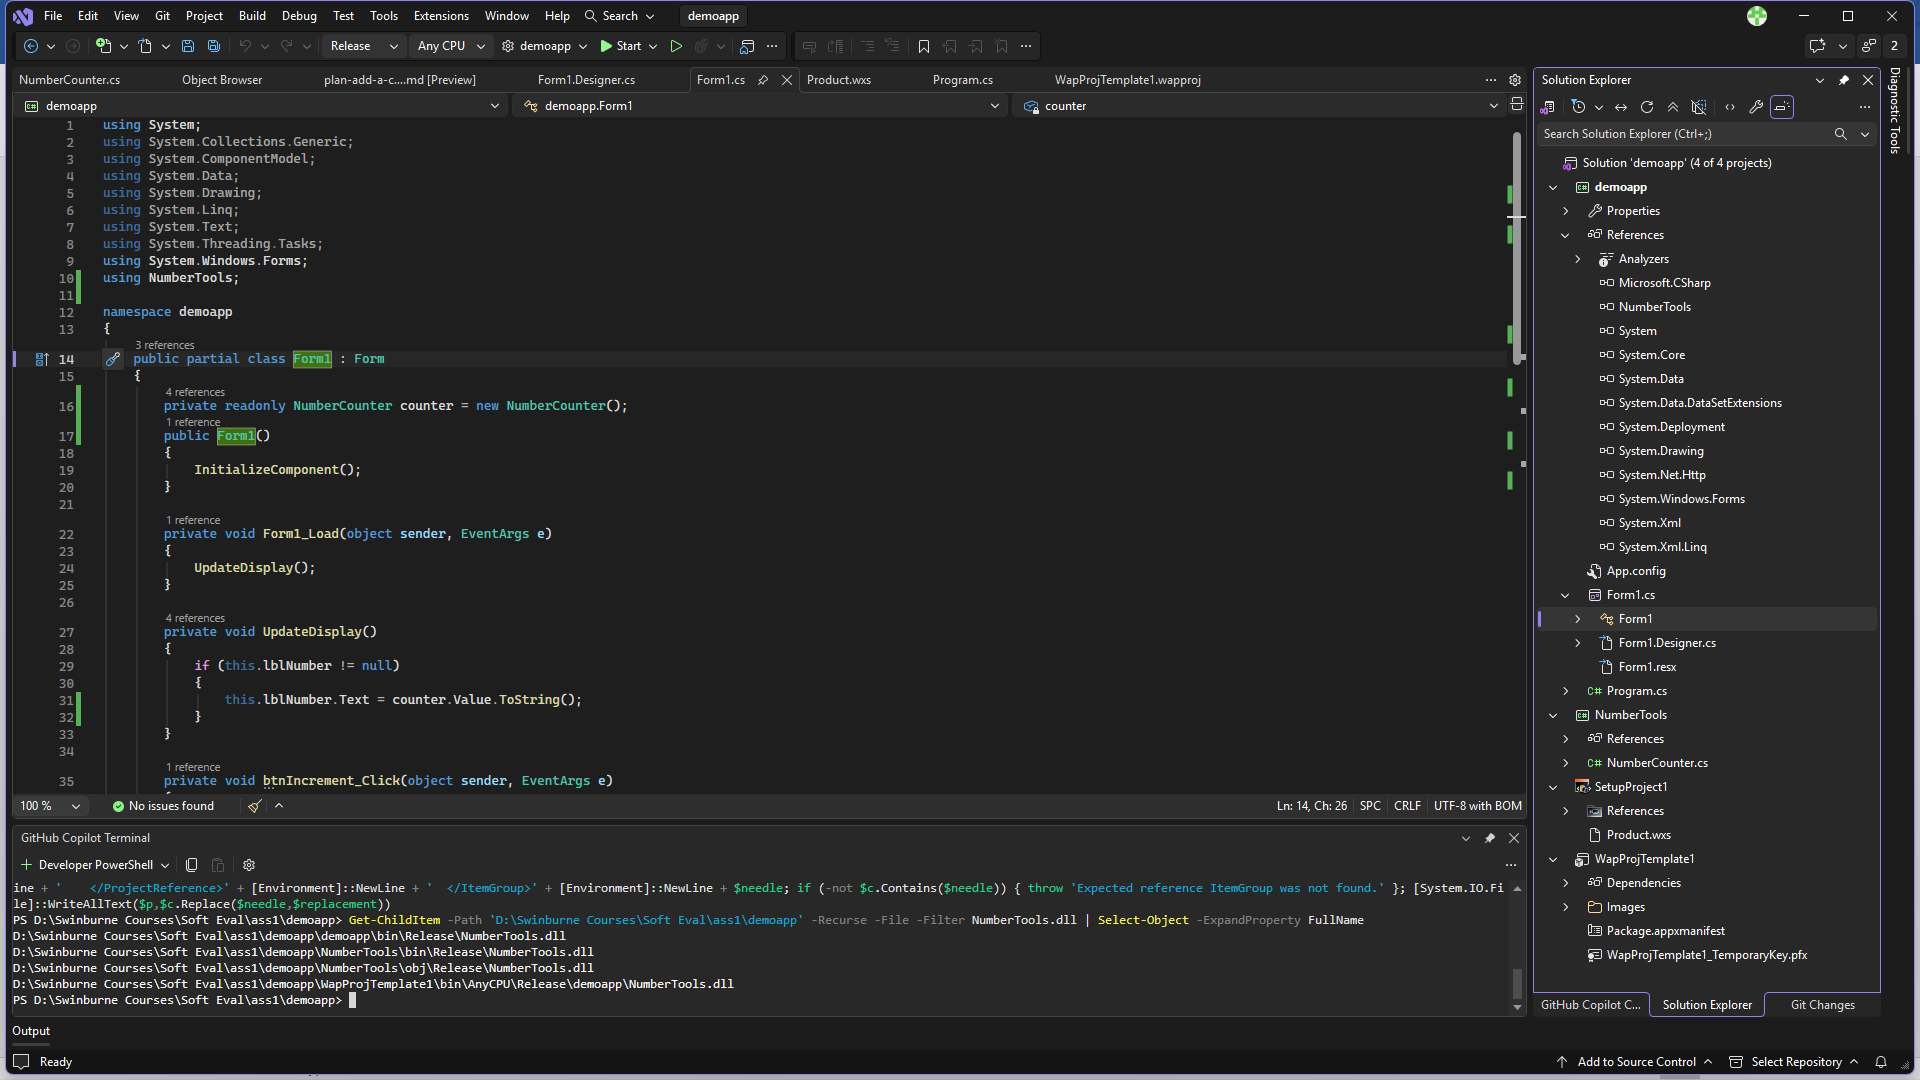
\includegraphics[width=\textwidth]{figures/image19.png}
        \caption{Refactored \texttt{Form1.cs} consuming the external DLL.}
        \label{fig:t3_new_code}
    \end{subfigure}
    \caption{Task 1.3 Implementation and Integration of Custom Dynamic-Link Library.}
    \label{fig:task3_evidence}
\end{figure}

\subsection{Multi-Component Deployment Packaging}
To deploy the multi-dependency application, both binaries must be packaged together:
\begin{itemize}[leftmargin=1.5cm]
    \item \textbf{WiX Configuration:} The \texttt{ComponentGroup} in \texttt{Product.wxs} was configured with distinct components for each file, assigning independent GUIDs:
\begin{lstlisting}[language=XML, caption={WiX Multi-Dependency Component Authoring}]
<ComponentGroup Id="ProductComponents" Directory="INSTALLFOLDER">
    <Component Id="demoapp.exe" Guid="f604d07c-f27a-46cb-99c1-11cc3c5db886">
        <File Id="demoapp.exe" Name="demoapp.exe" 
              Source="$(var.demoapp.TargetDir)demoapp.exe" KeyPath="yes" />
    </Component>
    <Component Id="NumberTools.dll" Guid="d82b4a11-8c43-4e6f-90e2-2a7b6cf0182e">
        <File Id="NumberTools.dll" Name="NumberTools.dll" 
              Source="$(var.demoapp.TargetDir)NumberTools.dll" KeyPath="yes" />
    </Component>
</ComponentGroup>
\end{lstlisting}
    \item \textbf{MSIX Package Layout:} In the Windows Application Packaging Project (\texttt{WapProjTemplate1}), the output bundle layout was inspected at \texttt{PackageLayout\textbackslash demoapp\textbackslash}. Both \texttt{demoapp.exe} and \texttt{NumberTools.dll} are packaged side-by-side, ensuring the OS loader resolves the DLL at application runtime.
\end{itemize}

\newpage

% --- Section 6: Task 1.4 ---
\section{Task 1.4 (High Distinction): Microsoft Store Deployment Pipeline}

\subsection{Step-by-Step Architecture for Microsoft Store Deployment}

\begin{figure}[H]
\centering
\begin{tcolorbox}[colback=codeBackground,colframe=navyBlue,title=\textbf{End-to-End Microsoft Store Publishing Pipeline}]
\small
\textbf{Step 1: Containerization via Windows Application Packaging (WAP)}
\begin{itemize}[leftmargin=0.5cm]
    \item Win32 desktop application (\texttt{demoapp.exe} + \texttt{NumberTools.dll}) is wrapped using Visual Studio's Windows Application Packaging Project.
    \item Visual assets (Square44x44, Square150x150, Wide310x150, StoreLogo) are generated and declared.
\end{itemize}
\textbf{Step 2: Manifest Configuration (\texttt{Package.appxmanifest})}
\begin{itemize}[leftmargin=0.5cm]
    \item Configure Package Identity (\texttt{Name}, \texttt{Publisher}, \texttt{Version}).
    \item Declare Application Capabilities (\texttt{runFullTrust} for desktop bridge interop).
\end{itemize}
\textbf{Step 3: Verification via Windows App Certification Kit (WACK)}
\begin{itemize}[leftmargin=0.5cm]
    \item Execute automated pre-submission tests: Security, Crashes and Hangs, App Manifest compliance, and Clean Removal tests.
\end{itemize}
\textbf{Step 4: Microsoft Partner Center Registration \& Submission}
\begin{itemize}[leftmargin=0.5cm]
    \item Register Microsoft Developer Account; reserve unique Application Name.
    \item Define Pricing, Market Availability, Age Ratings, and Storefront Promotional Descriptions.
\end{itemize}
\textbf{Step 5: Ingestion, Cloud Signing, and Public Store Release}
\begin{itemize}[leftmargin=0.5cm]
    \item Upload \texttt{.msixupload} bundle; Microsoft's ingestion pipeline validates binaries and re-signs the package with Microsoft's trusted root certificate.
\end{itemize}
\end{tcolorbox}
\caption{Architecture and Sequence of the Microsoft Store Deployment Process.}
\label{fig:store_pipeline}
\end{figure}

\subsection{Detailed Technical Stages}

\subsubsection{Stage 1: Manifest Authoring (\texttt{Package.appxmanifest})}
The packaging manifest acts as the security and runtime contract between the operating system and the packaged executable. It defines the application entry point, target architecture, and required execution permissions:

\begin{lstlisting}[language=XML, caption={Configured \texttt{Package.appxmanifest} Snippet}]
<Package xmlns="http://schemas.microsoft.com/appx/manifest/foundation/windows10"
         xmlns:uap="http://schemas.microsoft.com/appx/manifest/uap/windows10"
         xmlns:rescap="http://schemas.microsoft.com/appx/manifest/foundation/windows10/restrictedcapabilities">
  <Identity Name="DucThanhLe.DemoAppSoftEval"
            Publisher="CN=DucThanhLe, O=Swinburne, C=AU"
            Version="1.0.5.0" ProcessorArchitecture="x64" />
  <Applications>
    <Application Id="App" Executable="demoapp\demoapp.exe" EntryPoint="Windows.FullTrustApplication">
      <uap:VisualElements DisplayName="Demo App Soft Eval" 
                          Square150x150Logo="Images\Square150x150Logo.png" 
                          Square44x44Logo="Images\Square44x44Logo.png" 
                          Description="Step Counter Utility" BackgroundColor="transparent">
      </uap:VisualElements>
    </Application>
  </Applications>
  <Capabilities>
    <rescap:Capability Name="runFullTrust" />
  </Capabilities>
</Package>
\end{lstlisting}

\subsubsection{Stage 2: Package Signing and Code Trust Models}
During local prototyping and sideloading, the developer must generate a self-signed code-signing certificate (e.g., via PowerShell \texttt{New-SelfSignedCertificate}) and install it into the target machine's \texttt{Trusted People} certificate store. 

When deploying to the public Microsoft Store, however, the developer does \textbf{not} distribute their private certificate. Instead, Microsoft Partner Center strips any temporary developer signature during upload, runs automated malware/static analysis, and re-signs the MSIX payload with Microsoft's globally trusted CA root certificate. This guarantees that all Windows 10/11 machines worldwide will trust and install the application without user certificate warnings.

\subsubsection{Stage 3: Pre-Submission Validation via WACK}
Before submitting an application to Partner Center, it is mandatory to run the \textbf{Windows App Certification Kit (WACK)}. WACK evaluates the package against stringent OS compliance criteria:
\begin{enumerate}[leftmargin=1.2cm]
    \item \textbf{Crashes and Hangs Test:} Validates that the application does not trigger unhandled exceptions upon launch or during basic operational lifecycles.
    \item \textbf{App Capabilities Test:} Ensures that restricted capabilities like \texttt{runFullTrust} are strictly justified and do not access forbidden system boundaries.
    \item \textbf{Supported APIs Test:} Scans binary imports to guarantee that the application does not link against undocumented or deprecated Win32 private APIs.
    \item \textbf{Package Compliance:} Verifies manifest schema validity, valid XML namespaces, and complete image asset scaling (e.g., $100\%, 125\%, 150\%, 200\%$).
\end{enumerate}

\subsubsection{Stage 4: Partner Center Submission and Public Release}
Once certified locally, the submission workflow proceeds through the Microsoft Partner Center portal:
\begin{enumerate}[leftmargin=1.2cm]
    \item \textbf{App Name Reservation:} Under the developer dashboard, the unique name (e.g., \textit{DemoApp Soft Eval}) is reserved.
    \item \textbf{Pricing \& Availability:} Configure markets (Worldwide), pricing tier (Free), and discoverability settings.
    \item \textbf{Store Listings:} Provide promotional screenshots, descriptions, search keywords, and support contact details.
    \item \textbf{Package Upload:} The compiled \texttt{.msixupload} package (containing binaries and debugging symbols \texttt{.pdb}) is uploaded to the portal.
    \item \textbf{Automated Ingestion \& Certification:} Microsoft's cloud infrastructure executes automated tests, followed by final publication to the Microsoft Store within 24--48 hours.
\end{enumerate}

\newpage

% --- Section 8: Source Code and Scripts ---
\section{Source Code and Script Documentation}

\subsection{Public Repository Reference}
In accordance with rubric requirements, complete source files, Visual Studio solution files, WiX project definitions, and packaging manifests are published to a public repository for academic verification:
\begin{center}
\url{https://github.com/[YourUsername]/SWE40006-Portfolio-Task-1}
\end{center}

\subsection{Key Implementation Listings}

\subsubsection{WiX Setup Configuration (\texttt{Product.wxs})}
\begin{lstlisting}[language=XML, caption={\texttt{Product.wxs} WiX Deployment Configuration}]
<?xml version="1.0" encoding="UTF-8"?>
<Wix xmlns="http://schemas.microsoft.com/wix/2006/wi">
  <Product Id="*" Name="SetupProject1" Language="1033" Version="1.0.0.0" 
           Manufacturer="Duc Thanh Le" UpgradeCode="f04f5490-e571-4d6a-82c3-3705f07b5c6c">
    <Package InstallerVersion="200" Compressed="yes" InstallScope="perMachine" />

    <MajorUpgrade DowngradeErrorMessage="A newer version of [ProductName] is already installed." />
    <MediaTemplate EmbedCab="yes" />

    <Feature Id="ProductFeature" Title="SetupProject1" Level="1">
      <ComponentGroupRef Id="ProductComponents" />
    </Feature>
  </Product>

  <Fragment>
    <Directory Id="TARGETDIR" Name="SourceDir">
      <Directory Id="ProgramFilesFolder">
        <Directory Id="INSTALLFOLDER" Name="DemoAppSoftEval" />
      </Directory>
    </Directory>
  </Fragment>

  <Fragment>
    <ComponentGroup Id="ProductComponents" Directory="INSTALLFOLDER">
      <Component Id="demoapp.exe" Guid="f604d07c-f27a-46cb-99c1-11cc3c5db886">
        <File Id="demoapp.exe" Name="demoapp.exe" 
              Source="$(var.demoapp.TargetDir)demoapp.exe" KeyPath="yes" />
      </Component>
      <Component Id="NumberTools.dll" Guid="d82b4a11-8c43-4e6f-90e2-2a7b6cf0182e">
        <File Id="NumberTools.dll" Name="NumberTools.dll" 
              Source="$(var.demoapp.TargetDir)NumberTools.dll" KeyPath="yes" />
      </Component>
    </ComponentGroup>
  </Fragment>
</Wix>
\end{lstlisting}

\subsubsection{Client Form Presentation Logic (\texttt{Form1.cs})}
\begin{lstlisting}[language={[Sharp]C}, caption={\texttt{Form1.cs} Event Handling and Presentation Logic}, label={lst:form1}]
using System;
using System.Windows.Forms;
using NumberTools;

namespace demoapp
{
    public partial class Form1 : Form
    {
        private readonly NumberCounter counter = new NumberCounter();

        public Form1()
        {
            InitializeComponent();
        }

        private void Form1_Load(object sender, EventArgs e)
        {
            UpdateDisplay();
        }

        private void UpdateDisplay()
        {
            if (this.lblNumber != null)
            {
                this.lblNumber.Text = counter.Value.ToString();
            }
        }

        private void btnIncrement_Click(object sender, EventArgs e)
        {
            int step = 1;
            if (nudStep != null) step = (int)nudStep.Value;
            counter.Increment(step);
            UpdateDisplay();
        }

        private void btnDecrement_Click(object sender, EventArgs e)
        {
            int step = 1;
            if (nudStep != null) step = (int)nudStep.Value;
            counter.Decrement(step);
            UpdateDisplay();
        }

        private void btnReset_Click(object sender, EventArgs e)
        {
            counter.Reset();
            UpdateDisplay();
        }
    }
}
\end{lstlisting}
\end{document}
